\documentclass[]{book}
\usepackage{lmodern}
\usepackage{amssymb,amsmath}
\usepackage{ifxetex,ifluatex}
\usepackage{fixltx2e} % provides \textsubscript
\ifnum 0\ifxetex 1\fi\ifluatex 1\fi=0 % if pdftex
  \usepackage[T1]{fontenc}
  \usepackage[utf8]{inputenc}
\else % if luatex or xelatex
  \ifxetex
    \usepackage{mathspec}
  \else
    \usepackage{fontspec}
  \fi
  \defaultfontfeatures{Ligatures=TeX,Scale=MatchLowercase}
\fi
% use upquote if available, for straight quotes in verbatim environments
\IfFileExists{upquote.sty}{\usepackage{upquote}}{}
% use microtype if available
\IfFileExists{microtype.sty}{%
\usepackage{microtype}
\UseMicrotypeSet[protrusion]{basicmath} % disable protrusion for tt fonts
}{}
\usepackage[margin=1in]{geometry}
\usepackage{hyperref}
\hypersetup{unicode=true,
            pdftitle={life's work},
            pdfauthor={Charles T. Gray},
            pdfborder={0 0 0},
            breaklinks=true}
\urlstyle{same}  % don't use monospace font for urls
\usepackage{natbib}
\bibliographystyle{apalike}
\usepackage{color}
\usepackage{fancyvrb}
\newcommand{\VerbBar}{|}
\newcommand{\VERB}{\Verb[commandchars=\\\{\}]}
\DefineVerbatimEnvironment{Highlighting}{Verbatim}{commandchars=\\\{\}}
% Add ',fontsize=\small' for more characters per line
\usepackage{framed}
\definecolor{shadecolor}{RGB}{248,248,248}
\newenvironment{Shaded}{\begin{snugshade}}{\end{snugshade}}
\newcommand{\AlertTok}[1]{\textcolor[rgb]{0.94,0.16,0.16}{#1}}
\newcommand{\AnnotationTok}[1]{\textcolor[rgb]{0.56,0.35,0.01}{\textbf{\textit{#1}}}}
\newcommand{\AttributeTok}[1]{\textcolor[rgb]{0.77,0.63,0.00}{#1}}
\newcommand{\BaseNTok}[1]{\textcolor[rgb]{0.00,0.00,0.81}{#1}}
\newcommand{\BuiltInTok}[1]{#1}
\newcommand{\CharTok}[1]{\textcolor[rgb]{0.31,0.60,0.02}{#1}}
\newcommand{\CommentTok}[1]{\textcolor[rgb]{0.56,0.35,0.01}{\textit{#1}}}
\newcommand{\CommentVarTok}[1]{\textcolor[rgb]{0.56,0.35,0.01}{\textbf{\textit{#1}}}}
\newcommand{\ConstantTok}[1]{\textcolor[rgb]{0.00,0.00,0.00}{#1}}
\newcommand{\ControlFlowTok}[1]{\textcolor[rgb]{0.13,0.29,0.53}{\textbf{#1}}}
\newcommand{\DataTypeTok}[1]{\textcolor[rgb]{0.13,0.29,0.53}{#1}}
\newcommand{\DecValTok}[1]{\textcolor[rgb]{0.00,0.00,0.81}{#1}}
\newcommand{\DocumentationTok}[1]{\textcolor[rgb]{0.56,0.35,0.01}{\textbf{\textit{#1}}}}
\newcommand{\ErrorTok}[1]{\textcolor[rgb]{0.64,0.00,0.00}{\textbf{#1}}}
\newcommand{\ExtensionTok}[1]{#1}
\newcommand{\FloatTok}[1]{\textcolor[rgb]{0.00,0.00,0.81}{#1}}
\newcommand{\FunctionTok}[1]{\textcolor[rgb]{0.00,0.00,0.00}{#1}}
\newcommand{\ImportTok}[1]{#1}
\newcommand{\InformationTok}[1]{\textcolor[rgb]{0.56,0.35,0.01}{\textbf{\textit{#1}}}}
\newcommand{\KeywordTok}[1]{\textcolor[rgb]{0.13,0.29,0.53}{\textbf{#1}}}
\newcommand{\NormalTok}[1]{#1}
\newcommand{\OperatorTok}[1]{\textcolor[rgb]{0.81,0.36,0.00}{\textbf{#1}}}
\newcommand{\OtherTok}[1]{\textcolor[rgb]{0.56,0.35,0.01}{#1}}
\newcommand{\PreprocessorTok}[1]{\textcolor[rgb]{0.56,0.35,0.01}{\textit{#1}}}
\newcommand{\RegionMarkerTok}[1]{#1}
\newcommand{\SpecialCharTok}[1]{\textcolor[rgb]{0.00,0.00,0.00}{#1}}
\newcommand{\SpecialStringTok}[1]{\textcolor[rgb]{0.31,0.60,0.02}{#1}}
\newcommand{\StringTok}[1]{\textcolor[rgb]{0.31,0.60,0.02}{#1}}
\newcommand{\VariableTok}[1]{\textcolor[rgb]{0.00,0.00,0.00}{#1}}
\newcommand{\VerbatimStringTok}[1]{\textcolor[rgb]{0.31,0.60,0.02}{#1}}
\newcommand{\WarningTok}[1]{\textcolor[rgb]{0.56,0.35,0.01}{\textbf{\textit{#1}}}}
\usepackage{longtable,booktabs}
\usepackage{graphicx,grffile}
\makeatletter
\def\maxwidth{\ifdim\Gin@nat@width>\linewidth\linewidth\else\Gin@nat@width\fi}
\def\maxheight{\ifdim\Gin@nat@height>\textheight\textheight\else\Gin@nat@height\fi}
\makeatother
% Scale images if necessary, so that they will not overflow the page
% margins by default, and it is still possible to overwrite the defaults
% using explicit options in \includegraphics[width, height, ...]{}
\setkeys{Gin}{width=\maxwidth,height=\maxheight,keepaspectratio}
\IfFileExists{parskip.sty}{%
\usepackage{parskip}
}{% else
\setlength{\parindent}{0pt}
\setlength{\parskip}{6pt plus 2pt minus 1pt}
}
\setlength{\emergencystretch}{3em}  % prevent overfull lines
\providecommand{\tightlist}{%
  \setlength{\itemsep}{0pt}\setlength{\parskip}{0pt}}
\setcounter{secnumdepth}{5}
% Redefines (sub)paragraphs to behave more like sections
\ifx\paragraph\undefined\else
\let\oldparagraph\paragraph
\renewcommand{\paragraph}[1]{\oldparagraph{#1}\mbox{}}
\fi
\ifx\subparagraph\undefined\else
\let\oldsubparagraph\subparagraph
\renewcommand{\subparagraph}[1]{\oldsubparagraph{#1}\mbox{}}
\fi

%%% Use protect on footnotes to avoid problems with footnotes in titles
\let\rmarkdownfootnote\footnote%
\def\footnote{\protect\rmarkdownfootnote}

%%% Change title format to be more compact
\usepackage{titling}

% Create subtitle command for use in maketitle
\newcommand{\subtitle}[1]{
  \posttitle{
    \begin{center}\large#1\end{center}
    }
}

\setlength{\droptitle}{-2em}

  \title{life's work}
    \pretitle{\vspace{\droptitle}\centering\huge}
  \posttitle{\par}
    \author{Charles T. Gray}
    \preauthor{\centering\large\emph}
  \postauthor{\par}
      \predate{\centering\large\emph}
  \postdate{\par}
    \date{2019-03-20}

\usepackage{booktabs}

\begin{document}
\maketitle

{
\setcounter{tocdepth}{1}
\tableofcontents
}
\hypertarget{preamble}{%
\chapter{preamble}\label{preamble}}

What if one practices mathematical science like music?

My goal is to spend four hours a day on \emph{work with intent}\footnote{This term is adopted from a piano teacher that I studied under, that I subsequently adapted into my own teaching. She encouraged me to \emph{practice with intent}; that is, play what you intend to play. I found this to be particularly useful for discouraging my students, and myself, from the age-old pitfall of playing a piece of music until you make a mistake and stopping and playing that section over until you get it right. It's better to play \emph{through} the piece, which empBowers you to adapt to mistakes you will inevitably play and, most importantly, not lose time. Oddly, it appeared to be a universal misconception, myself included, that without careful consideration, the attempt to \emph{get the notes right} inevitably means the \textbf{rhythm is wrong}, and thus you get nothing right after all. Best, therefore, to play through the piece. I use my bullet journal to help me focus on work with intent; I've found the simplicity of only timing work when I've written down what I intend to do has been extraordinarily powerful in helping me complete daunting tasks.}.

For a sanity, efficiency, and inspiration, I intend to balance my time between three categories:

\begin{itemize}
\tightlist
\item
  research, \(\varphi\);
\item
  skills, \(\theta\); and
\item
  busywork, \(\psi\).
\end{itemize}

\hypertarget{analysis}{%
\chapter{analysis}\label{analysis}}

\hypertarget{workload-intensity}{%
\section{workload intensity}\label{workload-intensity}}

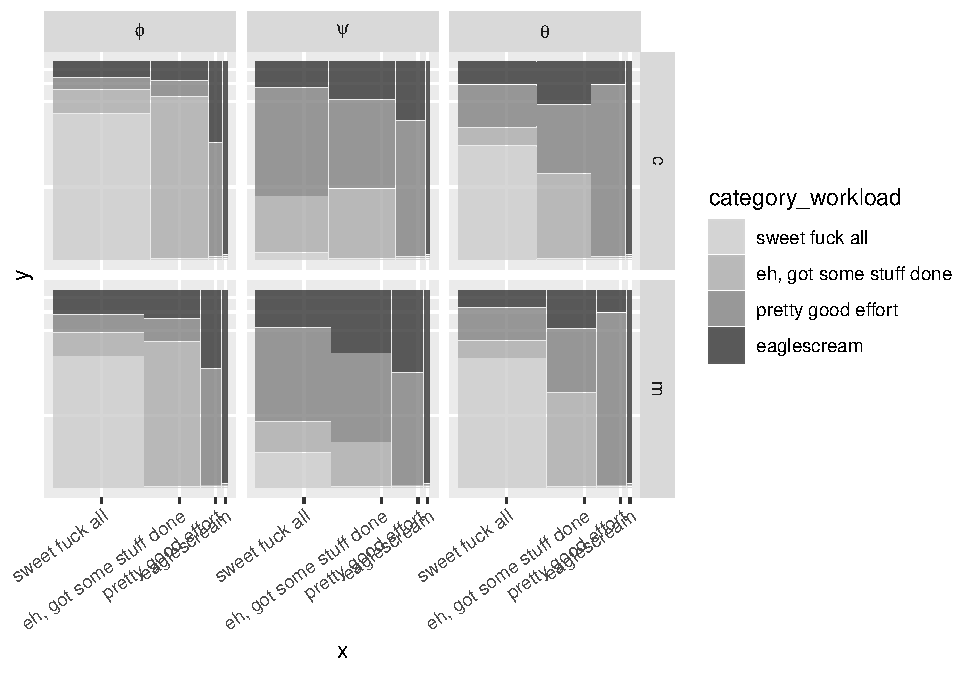
\includegraphics{lifeswork_files/figure-latex/vis-1.pdf}

\hypertarget{rituals}{%
\chapter{rituals}\label{rituals}}

\hypertarget{instantiate}{%
\section{instantiate}\label{instantiate}}

Start each \href{https://study.com/academy/lesson/german-days-of-the-week.html}{day} by drawing up a \protect\hyperlink{day-view}{day view}.

Begin the daily log, and add priority (\(*\)) \protect\hyperlink{daily-tasks}{daily tasks}.

\hypertarget{day-view}{%
\section{day view}\label{day-view}}

\begin{longtable}[]{@{}lll@{}}
\toprule
tracker & position & description\tabularnewline
\midrule
\endhead
poms & top left & track poms achieved\tabularnewline
goals & below poms & pom goals\tabularnewline
projects & top right & one project/category\tabularnewline
task cycles & below projects & \(\varphi, \theta, \psi, \overline o\)\tabularnewline
\protect\hyperlink{order-of-events}{order of events} & below goals & live with intent\tabularnewline
\bottomrule
\end{longtable}

\hypertarget{daily-tasks}{%
\section{daily tasks}\label{daily-tasks}}

\begin{tabular}{l|l|l|l|l}
\hline
priority & context & category & task & description\\
\hline
\$*\$ & \$\textbackslash{}forall\$ & \$\textbackslash{}psi\$ & what is on fire? & What must be advanced today or very bad things will happen? What things will make me feel less anxious or possibly awesome if I advance them?\\
\hline
\$*\$ & \$\textbackslash{}natural\$ & \$\textbackslash{}psi\$ & calendar & check day, week, month; note events of the day; upcoming deadlines\\
\hline
\$*\$ & \$\textbackslash{}natural\$ & \$\textbackslash{}psi\$ & inboxes & email, 3c2 , handbag, unpack suitcase\\
\hline
\$*\$ & \$\textbackslash{}sharp\$ & \$\textbackslash{}psi\$ & pill & take medication\\
\hline
\$\textbackslash{}sim\$ & \$\textbackslash{}forall\$ & \$\textbackslash{}psi\$ & monthly log & check list for anything that is on fire\\
\hline
\$\textbackslash{}sim\$ & \$\textbackslash{}natural\$ & \$\textbackslash{}psi\$ & needs action & finish pom\\
\hline
\$\textbackslash{}sim\$ & \$\textbackslash{}natural\$ & \$\textbackslash{}psi\$ & ynab & finish pom\\
\hline
\$\textbackslash{}varnothing\$ & \$\textbackslash{}natural\$ & \$\textbackslash{}pi\$ & dani & check in with dani on slack\\
\hline
\$\textbackslash{}varnothing\$ & \$\textbackslash{}natural\$ & \$\textbackslash{}psi\$ & waiting & waiting emails\\
\hline
\$\textbackslash{}varnothing\$ & \$\textbackslash{}natural\$ & \$\textbackslash{}theta\$ & export measures & download report into files, then email to myself, then download\\
\hline
\$\textbackslash{}varnothing\$ & \$\textbackslash{}sharp\$ & \$\textbackslash{}pi\$ & brushes & wash brushes\\
\hline
\$\textbackslash{}varnothing\$ & \$\textbackslash{}sharp\$ & \$\textbackslash{}pi\$ & kitchen & clean kitchen\\
\hline
\$\textbackslash{}varnothing\$ & \$\textbackslash{}sharp\$ & \$\textbackslash{}pi\$ & laundry & put away one basket of laundry\\
\hline
\$\textbackslash{}varnothing\$ & \$\textbackslash{}sharp\$ & \$\textbackslash{}pi\$ & floors & vacuum\\
\hline
\$\textbackslash{}varnothing\$ & \$\textbackslash{}sharp\$ & \$\textbackslash{}pi\$ & water plants & NA\\
\hline
\end{tabular}

\hypertarget{review}{%
\section{review}\label{review}}

\hypertarget{daily-log}{%
\subsection{daily log}\label{daily-log}}

Pare down to one active project per category and process daily log:

\begin{itemize}
\tightlist
\item
  migrate to GitHub issues or \protect\hyperlink{monthly-log}{monthly log}
\item
  add \protect\hyperlink{signifiers}{signifiers}
\item
  log projects in \protect\hyperlink{day-view}{day view} tracker
\item
  add projects from \protect\hyperlink{monthly-log}{monthly log} if all \(*\) and \(\sim\) have been completed
\end{itemize}

\hypertarget{day-view-1}{%
\subsection{day view}\label{day-view-1}}

\begin{itemize}
\tightlist
\item
  count poms
\item
  log goals
\item
  assign task cycles
\item
  +2 events to \protect\hyperlink{order-of-events}{order of events}
\end{itemize}

\hypertarget{minibreak-peeps}{%
\subsection{minibreak peeps}\label{minibreak-peeps}}

\begin{itemize}
\tightlist
\item
  social media \& slack
\end{itemize}

\hypertarget{monthly-log}{%
\section{monthly log}\label{monthly-log}}

List of projects that will take longer than a day.

\hypertarget{pom-goals}{%
\section{pom goals}\label{pom-goals}}

pom := 20 minutes

\begin{tabular}{l|r|r|r|r}
\hline
workload & phi & theta & psi & exercise\\
\hline
light & 2 & 1 & 1 & 1\\
\hline
moderate & 4 & 2 & 2 & 2\\
\hline
hardcore & 6 & 4 & 4 & 3\\
\hline
\end{tabular}

\hypertarget{order-of-events}{%
\section{order of events}\label{order-of-events}}

Day begins with \protect\hyperlink{review}{review} \(\overline o\).

\hypertarget{workday}{%
\subsection{workday}\label{workday}}

Alternate events:

\begin{itemize}
\tightlist
\item
  \(\not n + 2\) poms
\item
  \(\pi\)
\end{itemize}

Around other events such as meetings.

\hypertarget{wake-up}{%
\subsection{wake up}\label{wake-up}}

\begin{itemize}
\tightlist
\item
  wake up
\item
  {[}read{]}
\item
  dress
\item
  wash
\item
  {[}yoga{]}
\item
  \protect\hypertarget{day-view}{}{day view}
\item
  {[}yoga{]}
\end{itemize}

\hypertarget{evening}{%
\subsection{evening}\label{evening}}

\begin{itemize}
\tightlist
\item
  bathtime + reading
\item
  bed
\end{itemize}

\hypertarget{signifiers}{%
\section{signifiers}\label{signifiers}}

\begin{quote}
todo: create a signifiers sheet
\end{quote}

\begin{tabular}{l|l|r}
\hline
signifier & meaning & position\\
\hline
\$\textbackslash{}eigthnote\$ & today & 4\\
\hline
\$*\$ & priority & 5\\
\hline
\$i, ii, \textbackslash{}dots\$ & project & 4\\
\hline
\$\textbackslash{}sim\$ & anxiety & 5\\
\hline
\$\textbackslash{}cdot\$ & task & 1\\
\hline
\$\textbackslash{}varphi\$ & research & 2\\
\hline
\$\textbackslash{}theta\$ & skills & 2\\
\hline
\$\textbackslash{}psi\$ & busywork & 2\\
\hline
\$NA\$ & project & 3\\
\hline
\$NA\$ & look into & 3\\
\hline
\$\textbackslash{}natural\$ & on computer & 2\\
\hline
\$o\$ & event & 1\\
\hline
\$\textbackslash{}overline o\$ & review & 1\\
\hline
\$NA\$ & more than a day & 2\\
\hline
\end{tabular}

\hypertarget{ruminations}{%
\chapter{ruminations}\label{ruminations}}

\hypertarget{daily-projects}{%
\section{daily projects}\label{daily-projects}}

If a project is logged in the \protect\hypertarget{daily-log}{}{daily-log} then I am committing to finishing it today.

\hypertarget{pomodoros}{%
\section{pomodoros}\label{pomodoros}}

20 minutes seems to be the amount of time I can reasonably expect myself to focus unbroken.

\hypertarget{lowtech}{%
\section{lowtech}\label{lowtech}}

Keep what can be kept on paper, on paper. Keeps screens busy and helps me focus.

\hypertarget{section}{%
\section{}\label{section}}

\hypertarget{rmarkdown}{%
\chapter{rmarkdown}\label{rmarkdown}}

You can label chapter and section titles using \texttt{\{\#label\}} after them, e.g., we can reference Chapter \ref{intro}. If you do not manually label them, there will be automatic labels anyway, e.g., Chapter \ref{methods}.

Figures and tables with captions will be placed in \texttt{figure} and \texttt{table} environments, respectively.

\begin{Shaded}
\begin{Highlighting}[]
\KeywordTok{par}\NormalTok{(}\DataTypeTok{mar =} \KeywordTok{c}\NormalTok{(}\DecValTok{4}\NormalTok{, }\DecValTok{4}\NormalTok{, }\FloatTok{.1}\NormalTok{, }\FloatTok{.1}\NormalTok{))}
\KeywordTok{plot}\NormalTok{(pressure, }\DataTypeTok{type =} \StringTok{'b'}\NormalTok{, }\DataTypeTok{pch =} \DecValTok{19}\NormalTok{)}
\end{Highlighting}
\end{Shaded}

\begin{figure}

{\centering 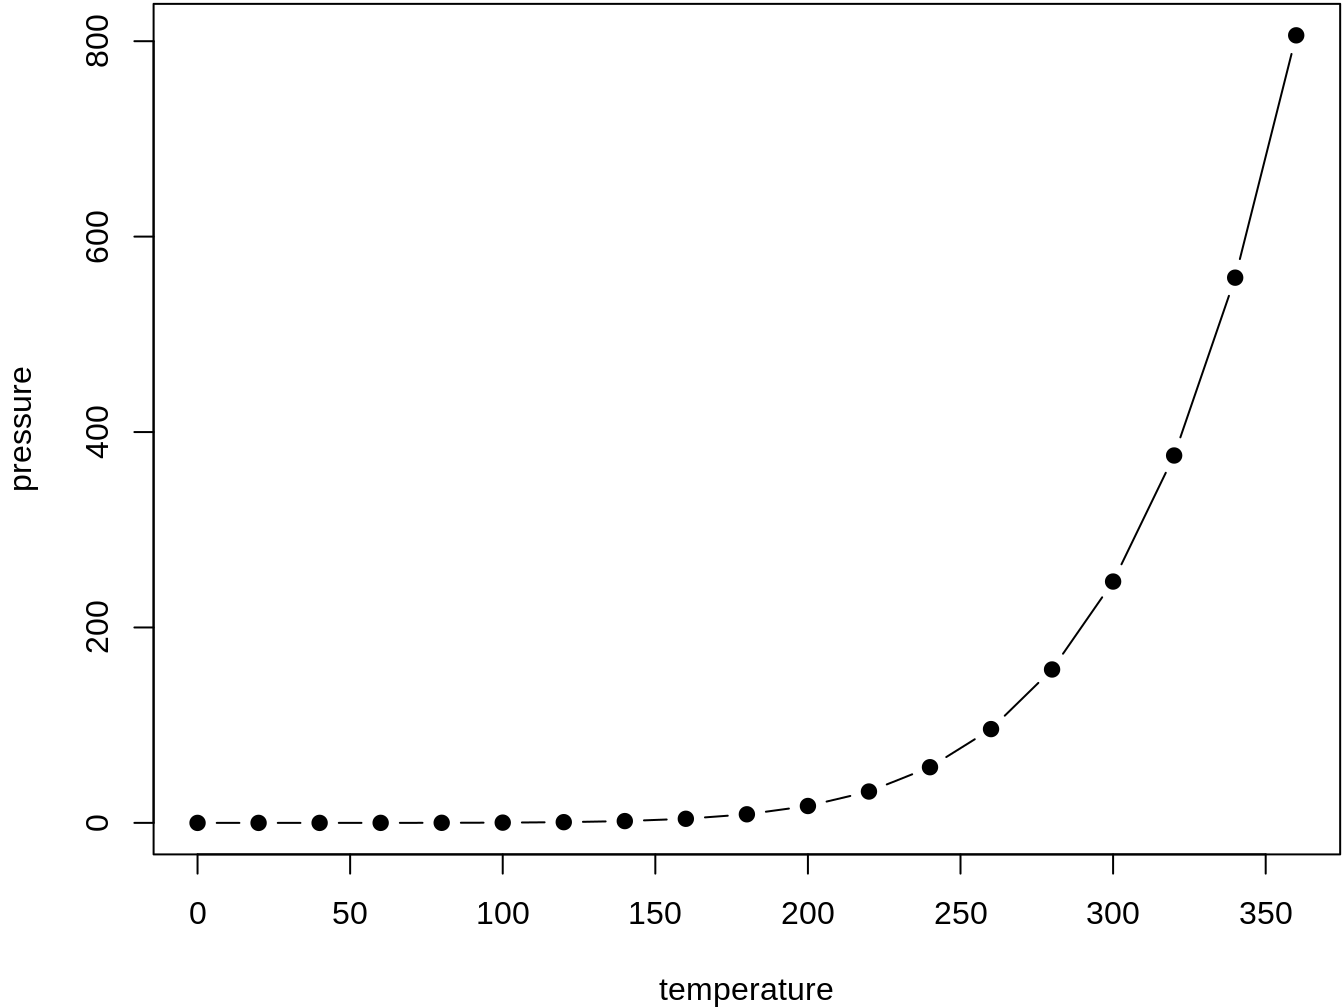
\includegraphics[width=0.8\linewidth]{lifeswork_files/figure-latex/nice-fig-1} 

}

\caption{Here is a nice figure!}\label{fig:nice-fig}
\end{figure}

Reference a figure by its code chunk label with the \texttt{fig:} prefix, e.g., see Figure \ref{fig:nice-fig}. Similarly, you can reference tables generated from \texttt{knitr::kable()}, e.g., see Table \ref{tab:nice-tab}.

\begin{Shaded}
\begin{Highlighting}[]
\NormalTok{knitr}\OperatorTok{::}\KeywordTok{kable}\NormalTok{(}
  \KeywordTok{head}\NormalTok{(iris, }\DecValTok{20}\NormalTok{), }\DataTypeTok{caption =} \StringTok{'Here is a nice table!'}\NormalTok{,}
  \DataTypeTok{booktabs =} \OtherTok{TRUE}
\NormalTok{)}
\end{Highlighting}
\end{Shaded}

\begin{table}

\caption{\label{tab:nice-tab}Here is a nice table!}
\centering
\begin{tabular}[t]{rrrrl}
\toprule
Sepal.Length & Sepal.Width & Petal.Length & Petal.Width & Species\\
\midrule
5.1 & 3.5 & 1.4 & 0.2 & setosa\\
4.9 & 3.0 & 1.4 & 0.2 & setosa\\
4.7 & 3.2 & 1.3 & 0.2 & setosa\\
4.6 & 3.1 & 1.5 & 0.2 & setosa\\
5.0 & 3.6 & 1.4 & 0.2 & setosa\\
\addlinespace
5.4 & 3.9 & 1.7 & 0.4 & setosa\\
4.6 & 3.4 & 1.4 & 0.3 & setosa\\
5.0 & 3.4 & 1.5 & 0.2 & setosa\\
4.4 & 2.9 & 1.4 & 0.2 & setosa\\
4.9 & 3.1 & 1.5 & 0.1 & setosa\\
\addlinespace
5.4 & 3.7 & 1.5 & 0.2 & setosa\\
4.8 & 3.4 & 1.6 & 0.2 & setosa\\
4.8 & 3.0 & 1.4 & 0.1 & setosa\\
4.3 & 3.0 & 1.1 & 0.1 & setosa\\
5.8 & 4.0 & 1.2 & 0.2 & setosa\\
\addlinespace
5.7 & 4.4 & 1.5 & 0.4 & setosa\\
5.4 & 3.9 & 1.3 & 0.4 & setosa\\
5.1 & 3.5 & 1.4 & 0.3 & setosa\\
5.7 & 3.8 & 1.7 & 0.3 & setosa\\
5.1 & 3.8 & 1.5 & 0.3 & setosa\\
\bottomrule
\end{tabular}
\end{table}

You can write citations, too. For example, we are using the \textbf{bookdown} package \citep{R-bookdown} in this sample book, which was built on top of R Markdown and \textbf{knitr} \citep{xie2015}.

\bibliography{book.bib,packages.bib}


\end{document}
